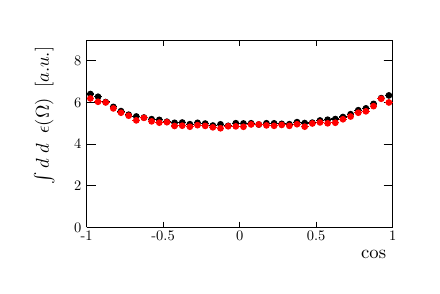
\begin{tikzpicture}
\pgfdeclareplotmark{cross} {
\pgfpathmoveto{\pgfpoint{-0.3\pgfplotmarksize}{\pgfplotmarksize}}
\pgfpathlineto{\pgfpoint{+0.3\pgfplotmarksize}{\pgfplotmarksize}}
\pgfpathlineto{\pgfpoint{+0.3\pgfplotmarksize}{0.3\pgfplotmarksize}}
\pgfpathlineto{\pgfpoint{+1\pgfplotmarksize}{0.3\pgfplotmarksize}}
\pgfpathlineto{\pgfpoint{+1\pgfplotmarksize}{-0.3\pgfplotmarksize}}
\pgfpathlineto{\pgfpoint{+0.3\pgfplotmarksize}{-0.3\pgfplotmarksize}}
\pgfpathlineto{\pgfpoint{+0.3\pgfplotmarksize}{-1.\pgfplotmarksize}}
\pgfpathlineto{\pgfpoint{-0.3\pgfplotmarksize}{-1.\pgfplotmarksize}}
\pgfpathlineto{\pgfpoint{-0.3\pgfplotmarksize}{-0.3\pgfplotmarksize}}
\pgfpathlineto{\pgfpoint{-1.\pgfplotmarksize}{-0.3\pgfplotmarksize}}
\pgfpathlineto{\pgfpoint{-1.\pgfplotmarksize}{0.3\pgfplotmarksize}}
\pgfpathlineto{\pgfpoint{-0.3\pgfplotmarksize}{0.3\pgfplotmarksize}}
\pgfpathclose
\pgfusepathqstroke
}
\pgfdeclareplotmark{cross*} {
\pgfpathmoveto{\pgfpoint{-0.3\pgfplotmarksize}{\pgfplotmarksize}}
\pgfpathlineto{\pgfpoint{+0.3\pgfplotmarksize}{\pgfplotmarksize}}
\pgfpathlineto{\pgfpoint{+0.3\pgfplotmarksize}{0.3\pgfplotmarksize}}
\pgfpathlineto{\pgfpoint{+1\pgfplotmarksize}{0.3\pgfplotmarksize}}
\pgfpathlineto{\pgfpoint{+1\pgfplotmarksize}{-0.3\pgfplotmarksize}}
\pgfpathlineto{\pgfpoint{+0.3\pgfplotmarksize}{-0.3\pgfplotmarksize}}
\pgfpathlineto{\pgfpoint{+0.3\pgfplotmarksize}{-1.\pgfplotmarksize}}
\pgfpathlineto{\pgfpoint{-0.3\pgfplotmarksize}{-1.\pgfplotmarksize}}
\pgfpathlineto{\pgfpoint{-0.3\pgfplotmarksize}{-0.3\pgfplotmarksize}}
\pgfpathlineto{\pgfpoint{-1.\pgfplotmarksize}{-0.3\pgfplotmarksize}}
\pgfpathlineto{\pgfpoint{-1.\pgfplotmarksize}{0.3\pgfplotmarksize}}
\pgfpathlineto{\pgfpoint{-0.3\pgfplotmarksize}{0.3\pgfplotmarksize}}
\pgfpathclose
\pgfusepathqfillstroke
}
\pgfdeclareplotmark{newstar} {
\pgfpathmoveto{\pgfqpoint{0pt}{\pgfplotmarksize}}
\pgfpathlineto{\pgfqpointpolar{44}{0.5\pgfplotmarksize}}
\pgfpathlineto{\pgfqpointpolar{18}{\pgfplotmarksize}}
\pgfpathlineto{\pgfqpointpolar{-20}{0.5\pgfplotmarksize}}
\pgfpathlineto{\pgfqpointpolar{-54}{\pgfplotmarksize}}
\pgfpathlineto{\pgfqpointpolar{-90}{0.5\pgfplotmarksize}}
\pgfpathlineto{\pgfqpointpolar{234}{\pgfplotmarksize}}
\pgfpathlineto{\pgfqpointpolar{198}{0.5\pgfplotmarksize}}
\pgfpathlineto{\pgfqpointpolar{162}{\pgfplotmarksize}}
\pgfpathlineto{\pgfqpointpolar{134}{0.5\pgfplotmarksize}}
\pgfpathclose
\pgfusepathqstroke
}
\pgfdeclareplotmark{newstar*} {
\pgfpathmoveto{\pgfqpoint{0pt}{\pgfplotmarksize}}
\pgfpathlineto{\pgfqpointpolar{44}{0.5\pgfplotmarksize}}
\pgfpathlineto{\pgfqpointpolar{18}{\pgfplotmarksize}}
\pgfpathlineto{\pgfqpointpolar{-20}{0.5\pgfplotmarksize}}
\pgfpathlineto{\pgfqpointpolar{-54}{\pgfplotmarksize}}
\pgfpathlineto{\pgfqpointpolar{-90}{0.5\pgfplotmarksize}}
\pgfpathlineto{\pgfqpointpolar{234}{\pgfplotmarksize}}
\pgfpathlineto{\pgfqpointpolar{198}{0.5\pgfplotmarksize}}
\pgfpathlineto{\pgfqpointpolar{162}{\pgfplotmarksize}}
\pgfpathlineto{\pgfqpointpolar{134}{0.5\pgfplotmarksize}}
\pgfpathclose
\pgfusepathqfillstroke
}
\definecolor{c}{rgb}{1,1,1};
\draw [color=c, fill=c] (5.1,3.20034) rectangle (9.9,6.21242);
\draw [color=c, fill=c] (5.772,3.68227) rectangle (9.66,6.06181);
\definecolor{c}{rgb}{0,0,0};
\draw [c] (5.772,3.68227) -- (5.772,6.06181) -- (9.66,6.06181) -- (9.66,3.68227) -- (5.772,3.68227);
\draw [c,line width=0.4] (5.8206,5.3665) -- (5.8206,5.37665);
\draw [c,line width=0.4] (5.8206,5.37665) -- (5.8206,5.3868);
\draw [c,line width=0.4] (5.772,5.37665) -- (5.8206,5.37665);
\draw [c,line width=0.4] (5.8206,5.37665) -- (5.8692,5.37665);
\foreach \P in {(5.8206,5.37665)}{\draw[mark options={color=c,fill=c},mark size=2.402402pt,mark=*,mark size=1pt] plot coordinates {\P};}
\draw [c,line width=0.4] (5.9178,5.33213) -- (5.9178,5.34217);
\draw [c,line width=0.4] (5.9178,5.34217) -- (5.9178,5.35222);
\draw [c,line width=0.4] (5.8692,5.34217) -- (5.9178,5.34217);
\draw [c,line width=0.4] (5.9178,5.34217) -- (5.9664,5.34217);
\foreach \P in {(5.9178,5.34217)}{\draw[mark options={color=c,fill=c},mark size=2.402402pt,mark=*,mark size=1pt] plot coordinates {\P};}
\draw [c,line width=0.4] (6.015,5.26518) -- (6.015,5.27502);
\draw [c,line width=0.4] (6.015,5.27502) -- (6.015,5.28486);
\draw [c,line width=0.4] (5.9664,5.27502) -- (6.015,5.27502);
\draw [c,line width=0.4] (6.015,5.27502) -- (6.0636,5.27502);
\foreach \P in {(6.015,5.27502)}{\draw[mark options={color=c,fill=c},mark size=2.402402pt,mark=*,mark size=1pt] plot coordinates {\P};}
\draw [c,line width=0.4] (6.1122,5.20394) -- (6.1122,5.21358);
\draw [c,line width=0.4] (6.1122,5.21358) -- (6.1122,5.22323);
\draw [c,line width=0.4] (6.0636,5.21358) -- (6.1122,5.21358);
\draw [c,line width=0.4] (6.1122,5.21358) -- (6.1608,5.21358);
\foreach \P in {(6.1122,5.21358)}{\draw[mark options={color=c,fill=c},mark size=2.402402pt,mark=*,mark size=1pt] plot coordinates {\P};}
\draw [c,line width=0.4] (6.2094,5.15027) -- (6.2094,5.15975);
\draw [c,line width=0.4] (6.2094,5.15975) -- (6.2094,5.16923);
\draw [c,line width=0.4] (6.1608,5.15975) -- (6.2094,5.15975);
\draw [c,line width=0.4] (6.2094,5.15975) -- (6.258,5.15975);
\foreach \P in {(6.2094,5.15975)}{\draw[mark options={color=c,fill=c},mark size=2.402402pt,mark=*,mark size=1pt] plot coordinates {\P};}
\draw [c,line width=0.4] (6.3066,5.10517) -- (6.3066,5.1145);
\draw [c,line width=0.4] (6.3066,5.1145) -- (6.3066,5.12383);
\draw [c,line width=0.4] (6.258,5.1145) -- (6.3066,5.1145);
\draw [c,line width=0.4] (6.3066,5.1145) -- (6.3552,5.1145);
\foreach \P in {(6.3066,5.1145)}{\draw[mark options={color=c,fill=c},mark size=2.402402pt,mark=*,mark size=1pt] plot coordinates {\P};}
\draw [c,line width=0.4] (6.4038,5.08243) -- (6.4038,5.09169);
\draw [c,line width=0.4] (6.4038,5.09169) -- (6.4038,5.10094);
\draw [c,line width=0.4] (6.3552,5.09169) -- (6.4038,5.09169);
\draw [c,line width=0.4] (6.4038,5.09169) -- (6.4524,5.09169);
\foreach \P in {(6.4038,5.09169)}{\draw[mark options={color=c,fill=c},mark size=2.402402pt,mark=*,mark size=1pt] plot coordinates {\P};}
\draw [c,line width=0.4] (6.501,5.06902) -- (6.501,5.07823);
\draw [c,line width=0.4] (6.501,5.07823) -- (6.501,5.08744);
\draw [c,line width=0.4] (6.4524,5.07823) -- (6.501,5.07823);
\draw [c,line width=0.4] (6.501,5.07823) -- (6.5496,5.07823);
\foreach \P in {(6.501,5.07823)}{\draw[mark options={color=c,fill=c},mark size=2.402402pt,mark=*,mark size=1pt] plot coordinates {\P};}
\draw [c,line width=0.4] (6.5982,5.04825) -- (6.5982,5.05739);
\draw [c,line width=0.4] (6.5982,5.05739) -- (6.5982,5.06654);
\draw [c,line width=0.4] (6.5496,5.05739) -- (6.5982,5.05739);
\draw [c,line width=0.4] (6.5982,5.05739) -- (6.6468,5.05739);
\foreach \P in {(6.5982,5.05739)}{\draw[mark options={color=c,fill=c},mark size=2.402402pt,mark=*,mark size=1pt] plot coordinates {\P};}
\draw [c,line width=0.4] (6.6954,5.03949) -- (6.6954,5.04861);
\draw [c,line width=0.4] (6.6954,5.04861) -- (6.6954,5.05772);
\draw [c,line width=0.4] (6.6468,5.04861) -- (6.6954,5.04861);
\draw [c,line width=0.4] (6.6954,5.04861) -- (6.744,5.04861);
\foreach \P in {(6.6954,5.04861)}{\draw[mark options={color=c,fill=c},mark size=2.402402pt,mark=*,mark size=1pt] plot coordinates {\P};}
\draw [c,line width=0.4] (6.7926,5.01639) -- (6.7926,5.02543);
\draw [c,line width=0.4] (6.7926,5.02543) -- (6.7926,5.03446);
\draw [c,line width=0.4] (6.744,5.02543) -- (6.7926,5.02543);
\draw [c,line width=0.4] (6.7926,5.02543) -- (6.8412,5.02543);
\foreach \P in {(6.7926,5.02543)}{\draw[mark options={color=c,fill=c},mark size=2.402402pt,mark=*,mark size=1pt] plot coordinates {\P};}
\draw [c,line width=0.4] (6.8898,5.00222) -- (6.8898,5.01121);
\draw [c,line width=0.4] (6.8898,5.01121) -- (6.8898,5.0202);
\draw [c,line width=0.4] (6.8412,5.01121) -- (6.8898,5.01121);
\draw [c,line width=0.4] (6.8898,5.01121) -- (6.9384,5.01121);
\foreach \P in {(6.8898,5.01121)}{\draw[mark options={color=c,fill=c},mark size=2.402402pt,mark=*,mark size=1pt] plot coordinates {\P};}
\draw [c,line width=0.4] (6.987,5.00594) -- (6.987,5.01495);
\draw [c,line width=0.4] (6.987,5.01495) -- (6.987,5.02395);
\draw [c,line width=0.4] (6.9384,5.01495) -- (6.987,5.01495);
\draw [c,line width=0.4] (6.987,5.01495) -- (7.0356,5.01495);
\foreach \P in {(6.987,5.01495)}{\draw[mark options={color=c,fill=c},mark size=2.402402pt,mark=*,mark size=1pt] plot coordinates {\P};}
\draw [c,line width=0.4] (7.0842,4.98471) -- (7.0842,4.99363);
\draw [c,line width=0.4] (7.0842,4.99363) -- (7.0842,5.00256);
\draw [c,line width=0.4] (7.0356,4.99363) -- (7.0842,4.99363);
\draw [c,line width=0.4] (7.0842,4.99363) -- (7.1328,4.99363);
\foreach \P in {(7.0842,4.99363)}{\draw[mark options={color=c,fill=c},mark size=2.402402pt,mark=*,mark size=1pt] plot coordinates {\P};}
\draw [c,line width=0.4] (7.1814,5.00232) -- (7.1814,5.01131);
\draw [c,line width=0.4] (7.1814,5.01131) -- (7.1814,5.02029);
\draw [c,line width=0.4] (7.1328,5.01131) -- (7.1814,5.01131);
\draw [c,line width=0.4] (7.1814,5.01131) -- (7.23,5.01131);
\foreach \P in {(7.1814,5.01131)}{\draw[mark options={color=c,fill=c},mark size=2.402402pt,mark=*,mark size=1pt] plot coordinates {\P};}
\draw [c,line width=0.4] (7.2786,4.99271) -- (7.2786,5.00167);
\draw [c,line width=0.4] (7.2786,5.00167) -- (7.2786,5.01062);
\draw [c,line width=0.4] (7.23,5.00167) -- (7.2786,5.00167);
\draw [c,line width=0.4] (7.2786,5.00167) -- (7.3272,5.00167);
\foreach \P in {(7.2786,5.00167)}{\draw[mark options={color=c,fill=c},mark size=2.402402pt,mark=*,mark size=1pt] plot coordinates {\P};}
\draw [c,line width=0.4] (7.3758,4.96784) -- (7.3758,4.97671);
\draw [c,line width=0.4] (7.3758,4.97671) -- (7.3758,4.98558);
\draw [c,line width=0.4] (7.3272,4.97671) -- (7.3758,4.97671);
\draw [c,line width=0.4] (7.3758,4.97671) -- (7.4244,4.97671);
\foreach \P in {(7.3758,4.97671)}{\draw[mark options={color=c,fill=c},mark size=2.402402pt,mark=*,mark size=1pt] plot coordinates {\P};}
\draw [c,line width=0.4] (7.473,4.98309) -- (7.473,4.99201);
\draw [c,line width=0.4] (7.473,4.99201) -- (7.473,5.00093);
\draw [c,line width=0.4] (7.4244,4.99201) -- (7.473,4.99201);
\draw [c,line width=0.4] (7.473,4.99201) -- (7.5216,4.99201);
\foreach \P in {(7.473,4.99201)}{\draw[mark options={color=c,fill=c},mark size=2.402402pt,mark=*,mark size=1pt] plot coordinates {\P};}
\draw [c,line width=0.4] (7.5702,4.9641) -- (7.5702,4.97296);
\draw [c,line width=0.4] (7.5702,4.97296) -- (7.5702,4.98181);
\draw [c,line width=0.4] (7.5216,4.97296) -- (7.5702,4.97296);
\draw [c,line width=0.4] (7.5702,4.97296) -- (7.6188,4.97296);
\foreach \P in {(7.5702,4.97296)}{\draw[mark options={color=c,fill=c},mark size=2.402402pt,mark=*,mark size=1pt] plot coordinates {\P};}
\draw [c,line width=0.4] (7.6674,4.99731) -- (7.6674,5.00628);
\draw [c,line width=0.4] (7.6674,5.00628) -- (7.6674,5.01525);
\draw [c,line width=0.4] (7.6188,5.00628) -- (7.6674,5.00628);
\draw [c,line width=0.4] (7.6674,5.00628) -- (7.716,5.00628);
\foreach \P in {(7.6674,5.00628)}{\draw[mark options={color=c,fill=c},mark size=2.402402pt,mark=*,mark size=1pt] plot coordinates {\P};}
\draw [c,line width=0.4] (7.7646,4.99426) -- (7.7646,5.00322);
\draw [c,line width=0.4] (7.7646,5.00322) -- (7.7646,5.01218);
\draw [c,line width=0.4] (7.716,5.00322) -- (7.7646,5.00322);
\draw [c,line width=0.4] (7.7646,5.00322) -- (7.8132,5.00322);
\foreach \P in {(7.7646,5.00322)}{\draw[mark options={color=c,fill=c},mark size=2.402402pt,mark=*,mark size=1pt] plot coordinates {\P};}
\draw [c,line width=0.4] (7.8618,4.99625) -- (7.8618,5.00522);
\draw [c,line width=0.4] (7.8618,5.00522) -- (7.8618,5.01419);
\draw [c,line width=0.4] (7.8132,5.00522) -- (7.8618,5.00522);
\draw [c,line width=0.4] (7.8618,5.00522) -- (7.9104,5.00522);
\foreach \P in {(7.8618,5.00522)}{\draw[mark options={color=c,fill=c},mark size=2.402402pt,mark=*,mark size=1pt] plot coordinates {\P};}
\draw [c,line width=0.4] (7.959,4.98055) -- (7.959,4.98946);
\draw [c,line width=0.4] (7.959,4.98946) -- (7.959,4.99837);
\draw [c,line width=0.4] (7.9104,4.98946) -- (7.959,4.98946);
\draw [c,line width=0.4] (7.959,4.98946) -- (8.0076,4.98946);
\foreach \P in {(7.959,4.98946)}{\draw[mark options={color=c,fill=c},mark size=2.402402pt,mark=*,mark size=1pt] plot coordinates {\P};}
\draw [c,line width=0.4] (8.0562,4.99645) -- (8.0562,5.00541);
\draw [c,line width=0.4] (8.0562,5.00541) -- (8.0562,5.01438);
\draw [c,line width=0.4] (8.0076,5.00541) -- (8.0562,5.00541);
\draw [c,line width=0.4] (8.0562,5.00541) -- (8.1048,5.00541);
\foreach \P in {(8.0562,5.00541)}{\draw[mark options={color=c,fill=c},mark size=2.402402pt,mark=*,mark size=1pt] plot coordinates {\P};}
\draw [c,line width=0.4] (8.1534,4.99565) -- (8.1534,5.00461);
\draw [c,line width=0.4] (8.1534,5.00461) -- (8.1534,5.01358);
\draw [c,line width=0.4] (8.1048,5.00461) -- (8.1534,5.00461);
\draw [c,line width=0.4] (8.1534,5.00461) -- (8.202,5.00461);
\foreach \P in {(8.1534,5.00461)}{\draw[mark options={color=c,fill=c},mark size=2.402402pt,mark=*,mark size=1pt] plot coordinates {\P};}
\draw [c,line width=0.4] (8.2506,4.98922) -- (8.2506,4.99816);
\draw [c,line width=0.4] (8.2506,4.99816) -- (8.2506,5.0071);
\draw [c,line width=0.4] (8.202,4.99816) -- (8.2506,4.99816);
\draw [c,line width=0.4] (8.2506,4.99816) -- (8.2992,4.99816);
\foreach \P in {(8.2506,4.99816)}{\draw[mark options={color=c,fill=c},mark size=2.402402pt,mark=*,mark size=1pt] plot coordinates {\P};}
\draw [c,line width=0.4] (8.3478,4.98446) -- (8.3478,4.99338);
\draw [c,line width=0.4] (8.3478,4.99338) -- (8.3478,5.00231);
\draw [c,line width=0.4] (8.2992,4.99338) -- (8.3478,4.99338);
\draw [c,line width=0.4] (8.3478,4.99338) -- (8.3964,4.99338);
\foreach \P in {(8.3478,4.99338)}{\draw[mark options={color=c,fill=c},mark size=2.402402pt,mark=*,mark size=1pt] plot coordinates {\P};}
\draw [c,line width=0.4] (8.445,5.01066) -- (8.445,5.01968);
\draw [c,line width=0.4] (8.445,5.01968) -- (8.445,5.02869);
\draw [c,line width=0.4] (8.3964,5.01968) -- (8.445,5.01968);
\draw [c,line width=0.4] (8.445,5.01968) -- (8.4936,5.01968);
\foreach \P in {(8.445,5.01968)}{\draw[mark options={color=c,fill=c},mark size=2.402402pt,mark=*,mark size=1pt] plot coordinates {\P};}
\draw [c,line width=0.4] (8.5422,4.99929) -- (8.5422,5.00827);
\draw [c,line width=0.4] (8.5422,5.00827) -- (8.5422,5.01725);
\draw [c,line width=0.4] (8.4936,5.00827) -- (8.5422,5.00827);
\draw [c,line width=0.4] (8.5422,5.00827) -- (8.5908,5.00827);
\foreach \P in {(8.5422,5.00827)}{\draw[mark options={color=c,fill=c},mark size=2.402402pt,mark=*,mark size=1pt] plot coordinates {\P};}
\draw [c,line width=0.4] (8.6394,5.00456) -- (8.6394,5.01356);
\draw [c,line width=0.4] (8.6394,5.01356) -- (8.6394,5.02255);
\draw [c,line width=0.4] (8.5908,5.01356) -- (8.6394,5.01356);
\draw [c,line width=0.4] (8.6394,5.01356) -- (8.688,5.01356);
\foreach \P in {(8.6394,5.01356)}{\draw[mark options={color=c,fill=c},mark size=2.402402pt,mark=*,mark size=1pt] plot coordinates {\P};}
\draw [c,line width=0.4] (8.7366,5.03177) -- (8.7366,5.04086);
\draw [c,line width=0.4] (8.7366,5.04086) -- (8.7366,5.04994);
\draw [c,line width=0.4] (8.688,5.04086) -- (8.7366,5.04086);
\draw [c,line width=0.4] (8.7366,5.04086) -- (8.7852,5.04086);
\foreach \P in {(8.7366,5.04086)}{\draw[mark options={color=c,fill=c},mark size=2.402402pt,mark=*,mark size=1pt] plot coordinates {\P};}
\draw [c,line width=0.4] (8.8338,5.04134) -- (8.8338,5.05046);
\draw [c,line width=0.4] (8.8338,5.05046) -- (8.8338,5.05958);
\draw [c,line width=0.4] (8.7852,5.05046) -- (8.8338,5.05046);
\draw [c,line width=0.4] (8.8338,5.05046) -- (8.8824,5.05046);
\foreach \P in {(8.8338,5.05046)}{\draw[mark options={color=c,fill=c},mark size=2.402402pt,mark=*,mark size=1pt] plot coordinates {\P};}
\draw [c,line width=0.4] (8.931,5.04989) -- (8.931,5.05904);
\draw [c,line width=0.4] (8.931,5.05904) -- (8.931,5.06819);
\draw [c,line width=0.4] (8.8824,5.05904) -- (8.931,5.05904);
\draw [c,line width=0.4] (8.931,5.05904) -- (8.9796,5.05904);
\foreach \P in {(8.931,5.05904)}{\draw[mark options={color=c,fill=c},mark size=2.402402pt,mark=*,mark size=1pt] plot coordinates {\P};}
\draw [c,line width=0.4] (9.0282,5.07575) -- (9.0282,5.08498);
\draw [c,line width=0.4] (9.0282,5.08498) -- (9.0282,5.09422);
\draw [c,line width=0.4] (8.9796,5.08498) -- (9.0282,5.08498);
\draw [c,line width=0.4] (9.0282,5.08498) -- (9.0768,5.08498);
\foreach \P in {(9.0282,5.08498)}{\draw[mark options={color=c,fill=c},mark size=2.402402pt,mark=*,mark size=1pt] plot coordinates {\P};}
\draw [c,line width=0.4] (9.1254,5.11106) -- (9.1254,5.12041);
\draw [c,line width=0.4] (9.1254,5.12041) -- (9.1254,5.12976);
\draw [c,line width=0.4] (9.0768,5.12041) -- (9.1254,5.12041);
\draw [c,line width=0.4] (9.1254,5.12041) -- (9.174,5.12041);
\foreach \P in {(9.1254,5.12041)}{\draw[mark options={color=c,fill=c},mark size=2.402402pt,mark=*,mark size=1pt] plot coordinates {\P};}
\draw [c,line width=0.4] (9.2226,5.16177) -- (9.2226,5.17128);
\draw [c,line width=0.4] (9.2226,5.17128) -- (9.2226,5.1808);
\draw [c,line width=0.4] (9.174,5.17128) -- (9.2226,5.17128);
\draw [c,line width=0.4] (9.2226,5.17128) -- (9.2712,5.17128);
\foreach \P in {(9.2226,5.17128)}{\draw[mark options={color=c,fill=c},mark size=2.402402pt,mark=*,mark size=1pt] plot coordinates {\P};}
\draw [c,line width=0.4] (9.3198,5.1853) -- (9.3198,5.19489);
\draw [c,line width=0.4] (9.3198,5.19489) -- (9.3198,5.20448);
\draw [c,line width=0.4] (9.2712,5.19489) -- (9.3198,5.19489);
\draw [c,line width=0.4] (9.3198,5.19489) -- (9.3684,5.19489);
\foreach \P in {(9.3198,5.19489)}{\draw[mark options={color=c,fill=c},mark size=2.402402pt,mark=*,mark size=1pt] plot coordinates {\P};}
\draw [c,line width=0.4] (9.417,5.24197) -- (9.417,5.25174);
\draw [c,line width=0.4] (9.417,5.25174) -- (9.417,5.26151);
\draw [c,line width=0.4] (9.3684,5.25174) -- (9.417,5.25174);
\draw [c,line width=0.4] (9.417,5.25174) -- (9.4656,5.25174);
\foreach \P in {(9.417,5.25174)}{\draw[mark options={color=c,fill=c},mark size=2.402402pt,mark=*,mark size=1pt] plot coordinates {\P};}
\draw [c,line width=0.4] (9.5142,5.31462) -- (9.5142,5.32461);
\draw [c,line width=0.4] (9.5142,5.32461) -- (9.5142,5.3346);
\draw [c,line width=0.4] (9.4656,5.32461) -- (9.5142,5.32461);
\draw [c,line width=0.4] (9.5142,5.32461) -- (9.5628,5.32461);
\foreach \P in {(9.5142,5.32461)}{\draw[mark options={color=c,fill=c},mark size=2.402402pt,mark=*,mark size=1pt] plot coordinates {\P};}
\draw [c,line width=0.4] (9.6114,5.34896) -- (9.6114,5.35905);
\draw [c,line width=0.4] (9.6114,5.35905) -- (9.6114,5.36915);
\draw [c,line width=0.4] (9.5628,5.35905) -- (9.6114,5.35905);
\draw [c,line width=0.4] (9.6114,5.35905) -- (9.66,5.35905);
\foreach \P in {(9.6114,5.35905)}{\draw[mark options={color=c,fill=c},mark size=2.402402pt,mark=*,mark size=1pt] plot coordinates {\P};}
\draw [c,line width=0.4] (5.772,3.68227) -- (9.66,3.68227);
\draw [anchor= east] (9.66,3.34492) node[scale=0.672711, rotate=0]{$\cos\thetamu$};
\draw [c,line width=0.4] (5.772,3.75546) -- (5.772,3.68227);
\draw [c,line width=0.4] (6.744,3.75546) -- (6.744,3.68227);
\draw [c,line width=0.4] (7.716,3.75546) -- (7.716,3.68227);
\draw [c,line width=0.4] (8.688,3.75546) -- (8.688,3.68227);
\draw [c,line width=0.4] (9.66,3.75546) -- (9.66,3.68227);
\draw [anchor=base] (5.772,3.51962) node[scale=0.52322, rotate=0]{-1};
\draw [anchor=base] (6.744,3.51962) node[scale=0.52322, rotate=0]{-0.5};
\draw [anchor=base] (7.716,3.51962) node[scale=0.52322, rotate=0]{0};
\draw [anchor=base] (8.688,3.51962) node[scale=0.52322, rotate=0]{0.5};
\draw [anchor=base] (9.66,3.51962) node[scale=0.52322, rotate=0]{1};
\draw [c,line width=0.4] (5.772,6.06181) -- (9.66,6.06181);
\draw [c,line width=0.4] (5.772,5.98862) -- (5.772,6.06181);
\draw [c,line width=0.4] (6.744,5.98862) -- (6.744,6.06181);
\draw [c,line width=0.4] (7.716,5.98862) -- (7.716,6.06181);
\draw [c,line width=0.4] (8.688,5.98862) -- (8.688,6.06181);
\draw [c,line width=0.4] (9.66,5.98862) -- (9.66,6.06181);
\draw [c,line width=0.4] (5.772,3.68227) -- (5.772,6.06181);
\draw [anchor= east] (5.2344,6.06181) node[scale=0.672711, rotate=90]{$\int d\thetaK \; d\phihel \;\; \epsilon(\Omega) \;\; [\text{a.u.}]$};
\draw [c,line width=0.4] (5.88576,3.68227) -- (5.772,3.68227);
\draw [c,line width=0.4] (5.88576,4.21106) -- (5.772,4.21106);
\draw [c,line width=0.4] (5.88576,4.73984) -- (5.772,4.73984);
\draw [c,line width=0.4] (5.88576,5.26863) -- (5.772,5.26863);
\draw [c,line width=0.4] (5.88576,5.79742) -- (5.772,5.79742);
\draw [c,line width=0.4] (5.88576,5.79742) -- (5.772,5.79742);
\draw [anchor= east] (5.772,3.68227) node[scale=0.52322, rotate=0]{0};
\draw [anchor= east] (5.772,4.21106) node[scale=0.52322, rotate=0]{2};
\draw [anchor= east] (5.772,4.73984) node[scale=0.52322, rotate=0]{4};
\draw [anchor= east] (5.772,5.26863) node[scale=0.52322, rotate=0]{6};
\draw [anchor= east] (5.772,5.79742) node[scale=0.52322, rotate=0]{8};
\draw [c,line width=0.4] (9.66,3.68227) -- (9.66,6.06181);
\draw [c,line width=0.4] (9.54624,3.68227) -- (9.66,3.68227);
\draw [c,line width=0.4] (9.54624,4.21106) -- (9.66,4.21106);
\draw [c,line width=0.4] (9.54624,4.73984) -- (9.66,4.73984);
\draw [c,line width=0.4] (9.54624,5.26863) -- (9.66,5.26863);
\draw [c,line width=0.4] (9.54624,5.79742) -- (9.66,5.79742);
\draw [c,line width=0.4] (9.54624,5.79742) -- (9.66,5.79742);
\definecolor{c}{rgb}{1,0,0};
\draw [c,line width=0.4] (5.8206,5.31071) -- (5.8206,5.32058);
\draw [c,line width=0.4] (5.8206,5.32058) -- (5.8206,5.33045);
\draw [c,line width=0.4] (5.772,5.32058) -- (5.8206,5.32058);
\draw [c,line width=0.4] (5.8206,5.32058) -- (5.8692,5.32058);
\foreach \P in {(5.8206,5.32058)}{\draw[mark options={color=c,fill=c},mark size=2.402402pt,mark=*,mark size=1pt] plot coordinates {\P};}
\draw [c,line width=0.4] (5.9178,5.26854) -- (5.9178,5.27828);
\draw [c,line width=0.4] (5.9178,5.27828) -- (5.9178,5.28803);
\draw [c,line width=0.4] (5.8692,5.27828) -- (5.9178,5.27828);
\draw [c,line width=0.4] (5.9178,5.27828) -- (5.9664,5.27828);
\foreach \P in {(5.9178,5.27828)}{\draw[mark options={color=c,fill=c},mark size=2.402402pt,mark=*,mark size=1pt] plot coordinates {\P};}
\draw [c,line width=0.4] (6.015,5.26023) -- (6.015,5.26995);
\draw [c,line width=0.4] (6.015,5.26995) -- (6.015,5.27967);
\draw [c,line width=0.4] (5.9664,5.26995) -- (6.015,5.26995);
\draw [c,line width=0.4] (6.015,5.26995) -- (6.0636,5.26995);
\foreach \P in {(6.015,5.26995)}{\draw[mark options={color=c,fill=c},mark size=2.402402pt,mark=*,mark size=1pt] plot coordinates {\P};}
\draw [c,line width=0.4] (6.1122,5.1845) -- (6.1122,5.19398);
\draw [c,line width=0.4] (6.1122,5.19398) -- (6.1122,5.20347);
\draw [c,line width=0.4] (6.0636,5.19398) -- (6.1122,5.19398);
\draw [c,line width=0.4] (6.1122,5.19398) -- (6.1608,5.19398);
\foreach \P in {(6.1122,5.19398)}{\draw[mark options={color=c,fill=c},mark size=2.402402pt,mark=*,mark size=1pt] plot coordinates {\P};}
\draw [c,line width=0.4] (6.2094,5.13018) -- (6.2094,5.13949);
\draw [c,line width=0.4] (6.2094,5.13949) -- (6.2094,5.1488);
\draw [c,line width=0.4] (6.1608,5.13949) -- (6.2094,5.13949);
\draw [c,line width=0.4] (6.2094,5.13949) -- (6.258,5.13949);
\foreach \P in {(6.2094,5.13949)}{\draw[mark options={color=c,fill=c},mark size=2.402402pt,mark=*,mark size=1pt] plot coordinates {\P};}
\draw [c,line width=0.4] (6.3066,5.09234) -- (6.3066,5.10153);
\draw [c,line width=0.4] (6.3066,5.10153) -- (6.3066,5.11072);
\draw [c,line width=0.4] (6.258,5.10153) -- (6.3066,5.10153);
\draw [c,line width=0.4] (6.3066,5.10153) -- (6.3552,5.10153);
\foreach \P in {(6.3066,5.10153)}{\draw[mark options={color=c,fill=c},mark size=2.402402pt,mark=*,mark size=1pt] plot coordinates {\P};}
\draw [c,line width=0.4] (6.4038,5.03311) -- (6.4038,5.0421);
\draw [c,line width=0.4] (6.4038,5.0421) -- (6.4038,5.05109);
\draw [c,line width=0.4] (6.3552,5.0421) -- (6.4038,5.0421);
\draw [c,line width=0.4] (6.4038,5.0421) -- (6.4524,5.0421);
\foreach \P in {(6.4038,5.0421)}{\draw[mark options={color=c,fill=c},mark size=2.402402pt,mark=*,mark size=1pt] plot coordinates {\P};}
\draw [c,line width=0.4] (6.501,5.0653) -- (6.501,5.0744);
\draw [c,line width=0.4] (6.501,5.0744) -- (6.501,5.0835);
\draw [c,line width=0.4] (6.4524,5.0744) -- (6.501,5.0744);
\draw [c,line width=0.4] (6.501,5.0744) -- (6.5496,5.0744);
\foreach \P in {(6.501,5.0744)}{\draw[mark options={color=c,fill=c},mark size=2.402402pt,mark=*,mark size=1pt] plot coordinates {\P};}
\draw [c,line width=0.4] (6.5982,5.02057) -- (6.5982,5.02952);
\draw [c,line width=0.4] (6.5982,5.02952) -- (6.5982,5.03848);
\draw [c,line width=0.4] (6.5496,5.02952) -- (6.5982,5.02952);
\draw [c,line width=0.4] (6.5982,5.02952) -- (6.6468,5.02952);
\foreach \P in {(6.5982,5.02952)}{\draw[mark options={color=c,fill=c},mark size=2.402402pt,mark=*,mark size=1pt] plot coordinates {\P};}
\draw [c,line width=0.4] (6.6954,5.00428) -- (6.6954,5.01318);
\draw [c,line width=0.4] (6.6954,5.01318) -- (6.6954,5.02207);
\draw [c,line width=0.4] (6.6468,5.01318) -- (6.6954,5.01318);
\draw [c,line width=0.4] (6.6954,5.01318) -- (6.744,5.01318);
\foreach \P in {(6.6954,5.01318)}{\draw[mark options={color=c,fill=c},mark size=2.402402pt,mark=*,mark size=1pt] plot coordinates {\P};}
\draw [c,line width=0.4] (6.7926,5.00991) -- (6.7926,5.01883);
\draw [c,line width=0.4] (6.7926,5.01883) -- (6.7926,5.02774);
\draw [c,line width=0.4] (6.744,5.01883) -- (6.7926,5.01883);
\draw [c,line width=0.4] (6.7926,5.01883) -- (6.8412,5.01883);
\foreach \P in {(6.7926,5.01883)}{\draw[mark options={color=c,fill=c},mark size=2.402402pt,mark=*,mark size=1pt] plot coordinates {\P};}
\draw [c,line width=0.4] (6.8898,4.9623) -- (6.8898,4.97105);
\draw [c,line width=0.4] (6.8898,4.97105) -- (6.8898,4.97981);
\draw [c,line width=0.4] (6.8412,4.97105) -- (6.8898,4.97105);
\draw [c,line width=0.4] (6.8898,4.97105) -- (6.9384,4.97105);
\foreach \P in {(6.8898,4.97105)}{\draw[mark options={color=c,fill=c},mark size=2.402402pt,mark=*,mark size=1pt] plot coordinates {\P};}
\draw [c,line width=0.4] (6.987,4.96582) -- (6.987,4.97459);
\draw [c,line width=0.4] (6.987,4.97459) -- (6.987,4.98336);
\draw [c,line width=0.4] (6.9384,4.97459) -- (6.987,4.97459);
\draw [c,line width=0.4] (6.987,4.97459) -- (7.0356,4.97459);
\foreach \P in {(6.987,4.97459)}{\draw[mark options={color=c,fill=c},mark size=2.402402pt,mark=*,mark size=1pt] plot coordinates {\P};}
\draw [c,line width=0.4] (7.0842,4.95272) -- (7.0842,4.96144);
\draw [c,line width=0.4] (7.0842,4.96144) -- (7.0842,4.97017);
\draw [c,line width=0.4] (7.0356,4.96144) -- (7.0842,4.96144);
\draw [c,line width=0.4] (7.0842,4.96144) -- (7.1328,4.96144);
\foreach \P in {(7.0842,4.96144)}{\draw[mark options={color=c,fill=c},mark size=2.402402pt,mark=*,mark size=1pt] plot coordinates {\P};}
\draw [c,line width=0.4] (7.1814,4.97229) -- (7.1814,4.98108);
\draw [c,line width=0.4] (7.1814,4.98108) -- (7.1814,4.98987);
\draw [c,line width=0.4] (7.1328,4.98108) -- (7.1814,4.98108);
\draw [c,line width=0.4] (7.1814,4.98108) -- (7.23,4.98108);
\foreach \P in {(7.1814,4.98108)}{\draw[mark options={color=c,fill=c},mark size=2.402402pt,mark=*,mark size=1pt] plot coordinates {\P};}
\draw [c,line width=0.4] (7.2786,4.96309) -- (7.2786,4.97185);
\draw [c,line width=0.4] (7.2786,4.97185) -- (7.2786,4.98061);
\draw [c,line width=0.4] (7.23,4.97185) -- (7.2786,4.97185);
\draw [c,line width=0.4] (7.2786,4.97185) -- (7.3272,4.97185);
\foreach \P in {(7.2786,4.97185)}{\draw[mark options={color=c,fill=c},mark size=2.402402pt,mark=*,mark size=1pt] plot coordinates {\P};}
\draw [c,line width=0.4] (7.3758,4.94539) -- (7.3758,4.95408);
\draw [c,line width=0.4] (7.3758,4.95408) -- (7.3758,4.96278);
\draw [c,line width=0.4] (7.3272,4.95408) -- (7.3758,4.95408);
\draw [c,line width=0.4] (7.3758,4.95408) -- (7.4244,4.95408);
\foreach \P in {(7.3758,4.95408)}{\draw[mark options={color=c,fill=c},mark size=2.402402pt,mark=*,mark size=1pt] plot coordinates {\P};}
\draw [c,line width=0.4] (7.473,4.93291) -- (7.473,4.94157);
\draw [c,line width=0.4] (7.473,4.94157) -- (7.473,4.95022);
\draw [c,line width=0.4] (7.4244,4.94157) -- (7.473,4.94157);
\draw [c,line width=0.4] (7.473,4.94157) -- (7.5216,4.94157);
\foreach \P in {(7.473,4.94157)}{\draw[mark options={color=c,fill=c},mark size=2.402402pt,mark=*,mark size=1pt] plot coordinates {\P};}
\draw [c,line width=0.4] (7.5702,4.95873) -- (7.5702,4.96748);
\draw [c,line width=0.4] (7.5702,4.96748) -- (7.5702,4.97622);
\draw [c,line width=0.4] (7.5216,4.96748) -- (7.5702,4.96748);
\draw [c,line width=0.4] (7.5702,4.96748) -- (7.6188,4.96748);
\foreach \P in {(7.5702,4.96748)}{\draw[mark options={color=c,fill=c},mark size=2.402402pt,mark=*,mark size=1pt] plot coordinates {\P};}
\draw [c,line width=0.4] (7.6674,4.9576) -- (7.6674,4.96634);
\draw [c,line width=0.4] (7.6674,4.96634) -- (7.6674,4.97508);
\draw [c,line width=0.4] (7.6188,4.96634) -- (7.6674,4.96634);
\draw [c,line width=0.4] (7.6674,4.96634) -- (7.716,4.96634);
\foreach \P in {(7.6674,4.96634)}{\draw[mark options={color=c,fill=c},mark size=2.402402pt,mark=*,mark size=1pt] plot coordinates {\P};}
\draw [c,line width=0.4] (7.7646,4.95226) -- (7.7646,4.96098);
\draw [c,line width=0.4] (7.7646,4.96098) -- (7.7646,4.9697);
\draw [c,line width=0.4] (7.716,4.96098) -- (7.7646,4.96098);
\draw [c,line width=0.4] (7.7646,4.96098) -- (7.8132,4.96098);
\foreach \P in {(7.7646,4.96098)}{\draw[mark options={color=c,fill=c},mark size=2.402402pt,mark=*,mark size=1pt] plot coordinates {\P};}
\draw [c,line width=0.4] (7.8618,4.98144) -- (7.8618,4.99026);
\draw [c,line width=0.4] (7.8618,4.99026) -- (7.8618,4.99908);
\draw [c,line width=0.4] (7.8132,4.99026) -- (7.8618,4.99026);
\draw [c,line width=0.4] (7.8618,4.99026) -- (7.9104,4.99026);
\foreach \P in {(7.8618,4.99026)}{\draw[mark options={color=c,fill=c},mark size=2.402402pt,mark=*,mark size=1pt] plot coordinates {\P};}
\draw [c,line width=0.4] (7.959,4.98166) -- (7.959,4.99048);
\draw [c,line width=0.4] (7.959,4.99048) -- (7.959,4.99931);
\draw [c,line width=0.4] (7.9104,4.99048) -- (7.959,4.99048);
\draw [c,line width=0.4] (7.959,4.99048) -- (8.0076,4.99048);
\foreach \P in {(7.959,4.99048)}{\draw[mark options={color=c,fill=c},mark size=2.402402pt,mark=*,mark size=1pt] plot coordinates {\P};}
\draw [c,line width=0.4] (8.0562,4.96942) -- (8.0562,4.9782);
\draw [c,line width=0.4] (8.0562,4.9782) -- (8.0562,4.98698);
\draw [c,line width=0.4] (8.0076,4.9782) -- (8.0562,4.9782);
\draw [c,line width=0.4] (8.0562,4.9782) -- (8.1048,4.9782);
\foreach \P in {(8.0562,4.9782)}{\draw[mark options={color=c,fill=c},mark size=2.402402pt,mark=*,mark size=1pt] plot coordinates {\P};}
\draw [c,line width=0.4] (8.1534,4.96417) -- (8.1534,4.97294);
\draw [c,line width=0.4] (8.1534,4.97294) -- (8.1534,4.9817);
\draw [c,line width=0.4] (8.1048,4.97294) -- (8.1534,4.97294);
\draw [c,line width=0.4] (8.1534,4.97294) -- (8.202,4.97294);
\foreach \P in {(8.1534,4.97294)}{\draw[mark options={color=c,fill=c},mark size=2.402402pt,mark=*,mark size=1pt] plot coordinates {\P};}
\draw [c,line width=0.4] (8.2506,4.97544) -- (8.2506,4.98424);
\draw [c,line width=0.4] (8.2506,4.98424) -- (8.2506,4.99304);
\draw [c,line width=0.4] (8.202,4.98424) -- (8.2506,4.98424);
\draw [c,line width=0.4] (8.2506,4.98424) -- (8.2992,4.98424);
\foreach \P in {(8.2506,4.98424)}{\draw[mark options={color=c,fill=c},mark size=2.402402pt,mark=*,mark size=1pt] plot coordinates {\P};}
\draw [c,line width=0.4] (8.3478,4.96394) -- (8.3478,4.9727);
\draw [c,line width=0.4] (8.3478,4.9727) -- (8.3478,4.98146);
\draw [c,line width=0.4] (8.2992,4.9727) -- (8.3478,4.9727);
\draw [c,line width=0.4] (8.3478,4.9727) -- (8.3964,4.9727);
\foreach \P in {(8.3478,4.9727)}{\draw[mark options={color=c,fill=c},mark size=2.402402pt,mark=*,mark size=1pt] plot coordinates {\P};}
\draw [c,line width=0.4] (8.445,4.98452) -- (8.445,4.99336);
\draw [c,line width=0.4] (8.445,4.99336) -- (8.445,5.00219);
\draw [c,line width=0.4] (8.3964,4.99336) -- (8.445,4.99336);
\draw [c,line width=0.4] (8.445,4.99336) -- (8.4936,4.99336);
\foreach \P in {(8.445,4.99336)}{\draw[mark options={color=c,fill=c},mark size=2.402402pt,mark=*,mark size=1pt] plot coordinates {\P};}
\draw [c,line width=0.4] (8.5422,4.95348) -- (8.5422,4.9622);
\draw [c,line width=0.4] (8.5422,4.9622) -- (8.5422,4.97093);
\draw [c,line width=0.4] (8.4936,4.9622) -- (8.5422,4.9622);
\draw [c,line width=0.4] (8.5422,4.9622) -- (8.5908,4.9622);
\foreach \P in {(8.5422,4.9622)}{\draw[mark options={color=c,fill=c},mark size=2.402402pt,mark=*,mark size=1pt] plot coordinates {\P};}
\draw [c,line width=0.4] (8.6394,4.99352) -- (8.6394,5.00238);
\draw [c,line width=0.4] (8.6394,5.00238) -- (8.6394,5.01125);
\draw [c,line width=0.4] (8.5908,5.00238) -- (8.6394,5.00238);
\draw [c,line width=0.4] (8.6394,5.00238) -- (8.688,5.00238);
\foreach \P in {(8.6394,5.00238)}{\draw[mark options={color=c,fill=c},mark size=2.402402pt,mark=*,mark size=1pt] plot coordinates {\P};}
\draw [c,line width=0.4] (8.7366,5.00712) -- (8.7366,5.01602);
\draw [c,line width=0.4] (8.7366,5.01602) -- (8.7366,5.02493);
\draw [c,line width=0.4] (8.688,5.01602) -- (8.7366,5.01602);
\draw [c,line width=0.4] (8.7366,5.01602) -- (8.7852,5.01602);
\foreach \P in {(8.7366,5.01602)}{\draw[mark options={color=c,fill=c},mark size=2.402402pt,mark=*,mark size=1pt] plot coordinates {\P};}
\draw [c,line width=0.4] (8.8338,4.99613) -- (8.8338,5.005);
\draw [c,line width=0.4] (8.8338,5.005) -- (8.8338,5.01387);
\draw [c,line width=0.4] (8.7852,5.005) -- (8.8338,5.005);
\draw [c,line width=0.4] (8.8338,5.005) -- (8.8824,5.005);
\foreach \P in {(8.8338,5.005)}{\draw[mark options={color=c,fill=c},mark size=2.402402pt,mark=*,mark size=1pt] plot coordinates {\P};}
\draw [c,line width=0.4] (8.931,5.00311) -- (8.931,5.012);
\draw [c,line width=0.4] (8.931,5.012) -- (8.931,5.0209);
\draw [c,line width=0.4] (8.8824,5.012) -- (8.931,5.012);
\draw [c,line width=0.4] (8.931,5.012) -- (8.9796,5.012);
\foreach \P in {(8.931,5.012)}{\draw[mark options={color=c,fill=c},mark size=2.402402pt,mark=*,mark size=1pt] plot coordinates {\P};}
\draw [c,line width=0.4] (9.0282,5.04716) -- (9.0282,5.0562);
\draw [c,line width=0.4] (9.0282,5.0562) -- (9.0282,5.06524);
\draw [c,line width=0.4] (8.9796,5.0562) -- (9.0282,5.0562);
\draw [c,line width=0.4] (9.0282,5.0562) -- (9.0768,5.0562);
\foreach \P in {(9.0282,5.0562)}{\draw[mark options={color=c,fill=c},mark size=2.402402pt,mark=*,mark size=1pt] plot coordinates {\P};}
\draw [c,line width=0.4] (9.1254,5.0818) -- (9.1254,5.09095);
\draw [c,line width=0.4] (9.1254,5.09095) -- (9.1254,5.10011);
\draw [c,line width=0.4] (9.0768,5.09095) -- (9.1254,5.09095);
\draw [c,line width=0.4] (9.1254,5.09095) -- (9.174,5.09095);
\foreach \P in {(9.1254,5.09095)}{\draw[mark options={color=c,fill=c},mark size=2.402402pt,mark=*,mark size=1pt] plot coordinates {\P};}
\draw [c,line width=0.4] (9.2226,5.13007) -- (9.2226,5.13938);
\draw [c,line width=0.4] (9.2226,5.13938) -- (9.2226,5.14869);
\draw [c,line width=0.4] (9.174,5.13938) -- (9.2226,5.13938);
\draw [c,line width=0.4] (9.2226,5.13938) -- (9.2712,5.13938);
\foreach \P in {(9.2226,5.13938)}{\draw[mark options={color=c,fill=c},mark size=2.402402pt,mark=*,mark size=1pt] plot coordinates {\P};}
\draw [c,line width=0.4] (9.3198,5.14782) -- (9.3198,5.15719);
\draw [c,line width=0.4] (9.3198,5.15719) -- (9.3198,5.16656);
\draw [c,line width=0.4] (9.2712,5.15719) -- (9.3198,5.15719);
\draw [c,line width=0.4] (9.3198,5.15719) -- (9.3684,5.15719);
\foreach \P in {(9.3198,5.15719)}{\draw[mark options={color=c,fill=c},mark size=2.402402pt,mark=*,mark size=1pt] plot coordinates {\P};}
\draw [c,line width=0.4] (9.417,5.2132) -- (9.417,5.22277);
\draw [c,line width=0.4] (9.417,5.22277) -- (9.417,5.23235);
\draw [c,line width=0.4] (9.3684,5.22277) -- (9.417,5.22277);
\draw [c,line width=0.4] (9.417,5.22277) -- (9.4656,5.22277);
\foreach \P in {(9.417,5.22277)}{\draw[mark options={color=c,fill=c},mark size=2.402402pt,mark=*,mark size=1pt] plot coordinates {\P};}
\draw [c,line width=0.4] (9.5142,5.3067) -- (9.5142,5.31656);
\draw [c,line width=0.4] (9.5142,5.31656) -- (9.5142,5.32643);
\draw [c,line width=0.4] (9.4656,5.31656) -- (9.5142,5.31656);
\draw [c,line width=0.4] (9.5142,5.31656) -- (9.5628,5.31656);
\foreach \P in {(9.5142,5.31656)}{\draw[mark options={color=c,fill=c},mark size=2.402402pt,mark=*,mark size=1pt] plot coordinates {\P};}
\draw [c,line width=0.4] (9.6114,5.2599) -- (9.6114,5.26962);
\draw [c,line width=0.4] (9.6114,5.26962) -- (9.6114,5.27934);
\draw [c,line width=0.4] (9.5628,5.26962) -- (9.6114,5.26962);
\draw [c,line width=0.4] (9.6114,5.26962) -- (9.66,5.26962);
\foreach \P in {(9.6114,5.26962)}{\draw[mark options={color=c,fill=c},mark size=2.402402pt,mark=*,mark size=1pt] plot coordinates {\P};}
\end{tikzpicture}
